\documentclass[12pt, a4paper]{article}
\usepackage[T2A]{fontenc}
\usepackage[utf8]{inputenc}
\usepackage[russian]{babel}
\usepackage{graphicx}
\usepackage{amsfonts}
\usepackage{indentfirst}
\usepackage{amsmath}
\usepackage{amsthm}
\usepackage{nicematrix}
\usepackage{hyperref}
\hypersetup{
    colorlinks=true,
    linkcolor=black,
    filecolor=magenta,      
    urlcolor=cyan,
    pdftitle={Lab4},
    pdfpagemode=FullScreen,
}
\usepackage{soulutf8}
\usepackage[left=1cm,right=1cm,
    top=2cm,bottom=2cm]{geometry}
\usepackage{titleps}
    \newpagestyle{main}{
        \setheadrule{0.4pt}
        \sethead{something}{\thepage}{}
}
\usepackage{listings}
\usepackage{color}

\definecolor{dkgreen}{rgb}{0,0.6,0}
\definecolor{gray}{rgb}{0.5,0.5,0.5}
\definecolor{mauve}{rgb}{0.58,0,0.82}

\lstset{frame=tb,
  language=Python,
  aboveskip=3mm,
  belowskip=3mm,
  showstringspaces=false,
  columns=flexible,
  basicstyle={\small\ttfamily},
  numbers=none,
  numberstyle=\tiny\color{gray},
  keywordstyle=\color{blue},
  commentstyle=\color{dkgreen},
  stringstyle=\color{mauve},
  breaklines=true,
  breakatwhitespace=true,
  tabsize=3
}
%\pagestyle{main}
\theoremstyle{plain}
\newtheorem{theorem}{Теорема}[section]
\newtheorem{corollary}{Следствие}[theorem]
\newtheorem*{example}{\textit{Пример}}
\newtheorem*{definition}{Определение}

\begin{document}
\begin{titlepage}
  \newpage
  \begin{center}
  \begin{tabular}{cc}
       \parbox{12cm}{\centering \textbf{НИУ ИТМО}}\\
       \\
       \hline
       \hline
  \end{tabular}
  \end{center}

  \begin{center}
  \caps{\textbf{Факультет систем управления и робототехники}}\\ 
  \end{center}
  
  \vspace{1cm}
  
  \begin{center}
      \textsc{Лабораторная работа № 2\\ по дисциплине <<Частотные методы>>}
  \end{center}
  
  \vspace{8em}
  
  \noindent Выполнил:  \hfill Гридусов Д.Д
  
  \vspace{20pt}
  \noindent Преподаватель: \hfill Перегудин А.А \\
  \\
  \vfill
  \begin{center}
  Санкт-Петербург \\2024 г.
  \end{center}
  
  \end{titlepage}
  
  \tableofcontents
  \newpage
  \section{Вещественное}
  \subsection{Прямоугольная функция}
  \[
  f_1(t) =  \begin{cases}
    a, |t| \leq b,\\
    0, |t| > b
  \end{cases}
  \]
  \noindent С помощью унитарного преобразования к угловой частоте найдем образ Фурье:
  \\
  \begin{center}
  $c_1(\omega) = \frac{1}{\sqrt{2\pi}} \int\limits_{-\infty}^{+\infty}f(t)e^{-i\omega t}dt = \frac{1}{\sqrt{2\pi}}\int\limits_{-b}^b a e^{-i\omega t} = 
  \frac{a}{\sqrt{2 \pi}} (\frac{e^{-iwt}}{-i\omega}|_{-b}^b) = \frac{a}{\sqrt{2 \pi}} \frac{e^{i\omega b} - e^{-i\omega b}}{i\omega} = \frac{a}{\sqrt{2 \pi}} \frac{2\sin(\omega b)}{w}  = \frac{2a \sin(\omega b)}{\sqrt{2 \pi} \omega}
  $ 
  \end{center}
\noindent Теперь построим графики Фурье образа и самой функции при различных значениях a и b.
\begin{figure}[!htb]
  \minipage{0.32\textwidth}
    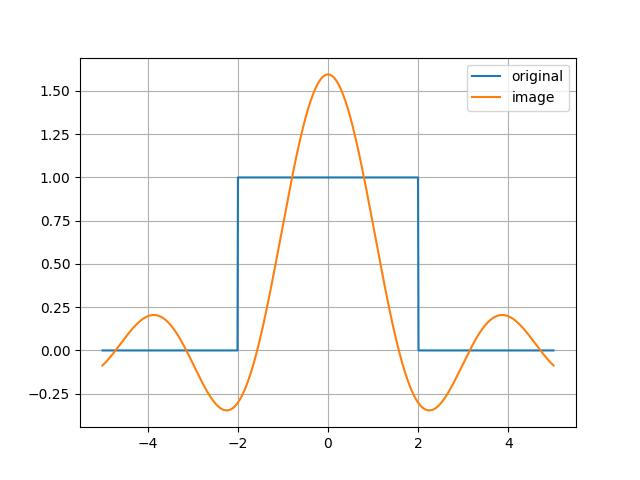
\includegraphics[width=\linewidth]{../image/sqWave_1_2.jpg}
    \caption{a = 1, b = 2}
  \endminipage\hfill
  \minipage{0.32\textwidth}
    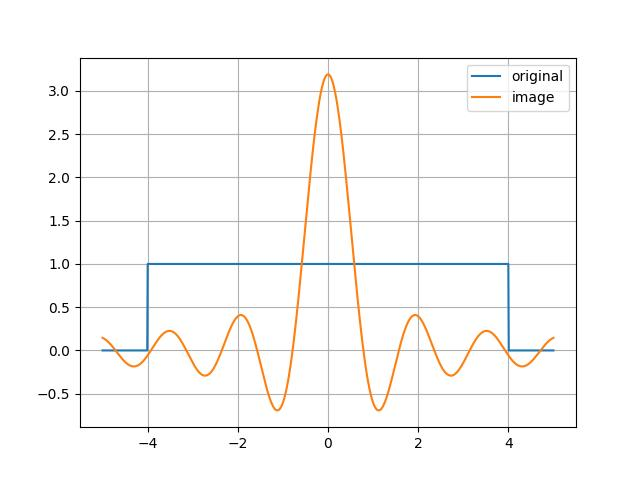
\includegraphics[width=\linewidth]{../image/sqWave_1_4.jpg}
    \caption{a = 1, b = 4}
  \endminipage\hfill
  \minipage{0.32\textwidth}%
    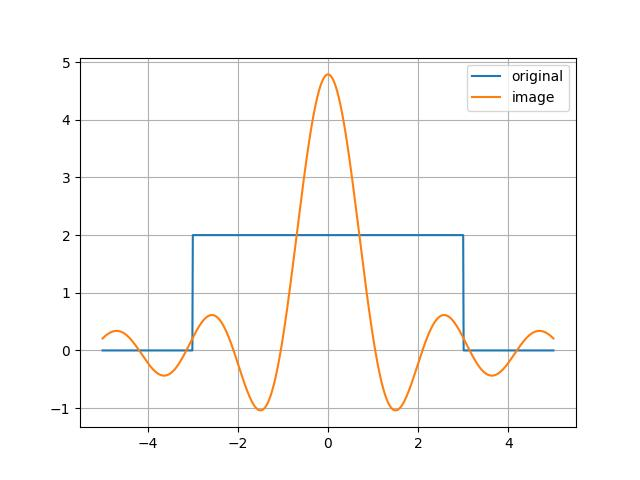
\includegraphics[width=\linewidth]{../image/sqWave_2_3.jpg}
    \caption{a = 2, b = 3}
  \endminipage
  \end{figure}
  
  \noindent \textbf{Равенство Парсеваля:}\\
  
  \begin{center}
    $\parallel f \parallel^2 = \int\limits_{-b}^{b} f^2(t) dt= [a = 1, b = 3] = 6$
  \end{center}
  \begin{center}
    $\parallel c(\omega)\parallel^ 2 = \int\limits_{-\infty}^{\infty}c^2(\omega)d\omega = 6 $
  \end{center}
  \subsection{Треугольная функция}
  \[
  f_2(t) =  \begin{cases}
    a - |\frac{a}{b}t|, |t| \leq b,\\
    0, |t| > b
  \end{cases}
  \]
  \textbf{Образ Фурье:}  \\
  \begin{center}
    $c_2(\omega) = \frac{1}{\sqrt{2\pi}} \int\limits_{-\infty}^{+\infty}f(t)e^{-i\omega t}dt = 
  \frac{1}{\sqrt{2\pi}}(\int\limits_{-b}^{0}(a + \frac{a}{b}t)e^{-iwt} + \int\limits_0^{b} (a - \frac{a}{b}t)e^{-iwt}dt) = -\frac{\sqrt{2}a(\cos(b\omega) - 1)}{b\omega^2}
  $
  \end{center}
  \begin{figure}[!htb]
    \minipage{0.32\textwidth}
      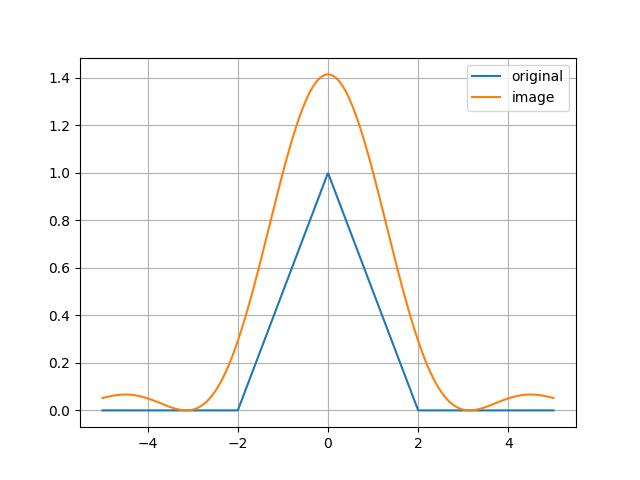
\includegraphics[width=\linewidth]{../image/trWave_1_2.jpg}
      \caption{$a=1$, $b=2$}
    \endminipage\hfill
    \minipage{0.32\textwidth}
      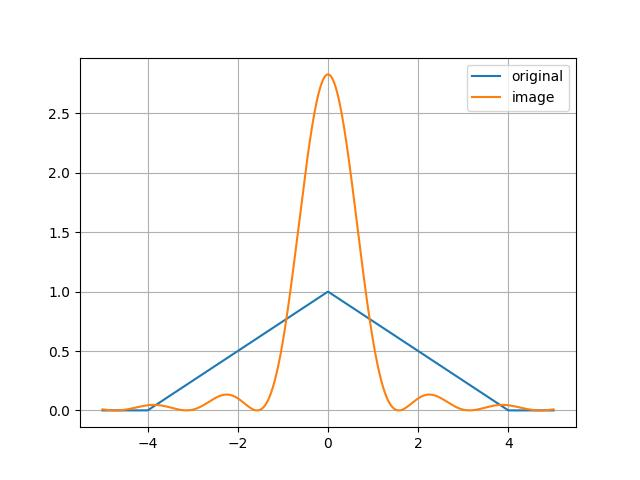
\includegraphics[width=\linewidth]{../image/trWave_1_4.jpg}
      \caption{$a = 1$, $b = 4$}
    \endminipage\hfill
    \minipage{0.32\textwidth}%
      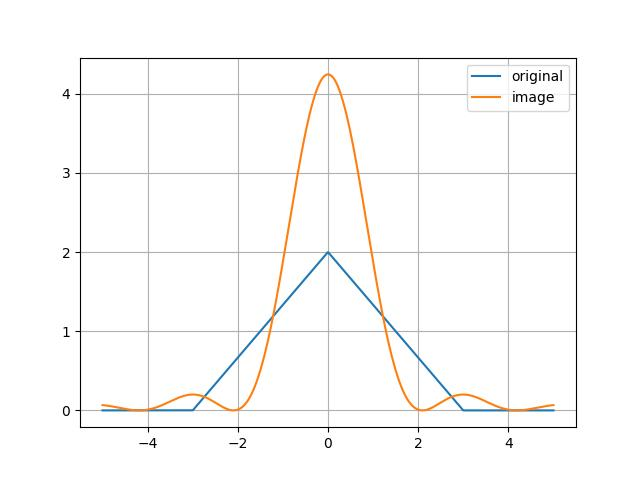
\includegraphics[width=\linewidth]{../image/trWave_2_3.jpg}
      \caption{$a = 2$, $b = 3$}
    \endminipage
    \end{figure}

  \subsection{Кардинальный синус}
  \[
  f_3(t) =  
    a \frac{\sin(\pi bt)}{\pi bt}
  \]
  \textbf{Образ Фурье: }
  \\
  \begin{center}
    $c_3(\omega) = \frac{1}{\sqrt{2\pi}} \int\limits_{-\infty}^{+\infty}f(t)e^{-i\omega t}dt = 
  \frac{a}{\sqrt{2\pi}b\pi}\int\limits_{-\infty}^{+\infty} \frac{e^{i\pi bt} - e^{-i\pi bt} }{2it}e^{-iwt} dt=
  \frac{a}{\sqrt{2\pi} b \pi} \int \limits_{-\infty}^{+\infty}\frac{e^{(\pi b-\omega)it} - e^{-(\pi b+\omega)it}}{2i t}dt
  $
  \end{center}
  \noindent Если не останавливаться, разбить на два и проигнтегрировать каждый по частым, то в итоге должна получиться уже знакомая нам прямоугольная функция.\\
  \[c_3(\omega) = 
  \begin{cases}
    \frac{a}{b\sqrt{2 \pi}}, |\omega| \leq b\pi,\\
    0, |\omega| > b\pi
  \end{cases}
  \]
  \textbf{Равенство Парсеваля:}
  \begin{center}
    $\parallel f \parallel^2 = \int\limits_{-\infty}^{+\infty} f^2(t) dt= [a = 1, b = 3] = \frac{1}{3}  $
  \end{center}
  \begin{center}
    $\parallel c(\omega)\parallel^ 2 = \int\limits_{-\infty}^{\infty}c^2(\omega)d\omega = \frac{1}{3} $
  \end{center}
  \begin{figure}[!htb]
    \minipage{0.32\textwidth}
      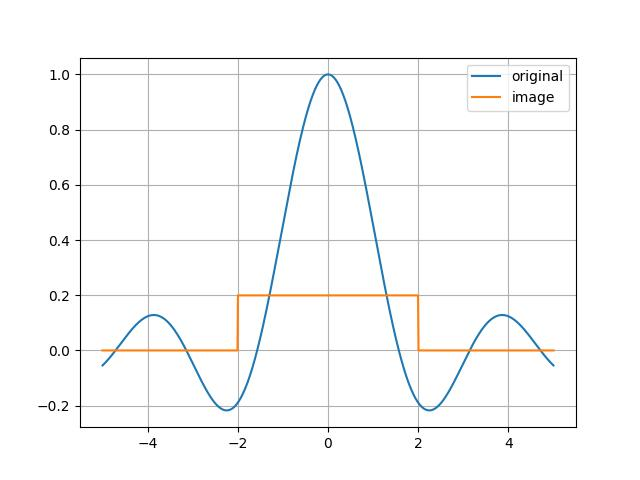
\includegraphics[width=\linewidth]{../image/cardinal_sinus_1_2}
      \caption{$a=1$, $b=2$}
    \endminipage\hfill
    \minipage{0.32\textwidth}
      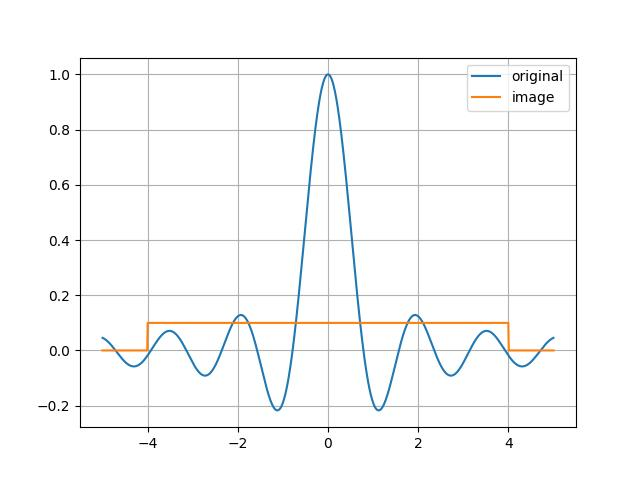
\includegraphics[width=\linewidth]{../image/cardinal_sinus_1_4.jpg}
      \caption{$a = 1$, $b = 4$}
    \endminipage\hfill
    \minipage{0.32\textwidth}%
      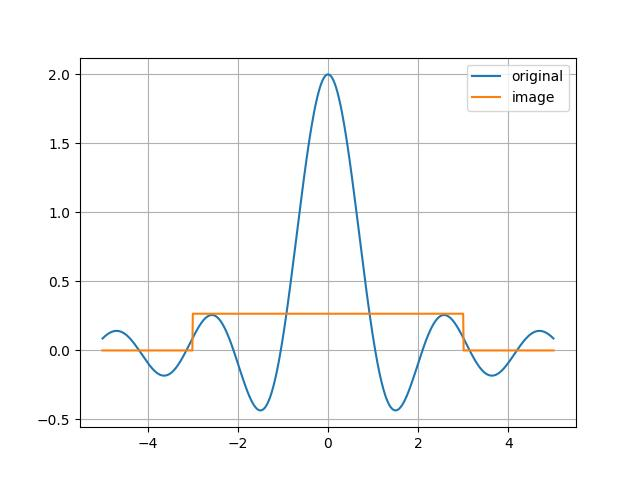
\includegraphics[width=\linewidth]{../image/cardinal_sinus_2_3.jpg}
      \caption{$a = 2$, $b = 3$}
    \endminipage
    \end{figure}
  \subsection{Функция Гаусса}
  \[
  f_4(t) = 
    a e^{-bt^2}
  \]
  \textbf{Образ Фурье:}  \\
  \begin{center}
    $c_4(\omega) = \frac{1}{\sqrt{2\pi}} \int\limits_{-\infty}^{+\infty}f(t)e^{-i\omega t}dt = 
  \frac{1}{\sqrt{2\pi}} a \int\limits_{-\infty}^{+\infty} e^{-bt^2 - iwt}dt = 
  \frac{a}{\sqrt{2 b}} e^{-\frac{\omega^2}{4b}}
  $ 
  \end{center} 
\noindent \textbf{Равенство Парсеваля}
\begin{center}
  $\parallel f \parallel^2 = \int\limits_{-\infty}^{+\infty} f^2(t) dt= [a = 1, b = 3] = 0.724  $
\end{center}
\begin{center}
  $\parallel c(\omega)\parallel^ 2 = \int\limits_{-\infty}^{\infty}c^2(\omega)d\omega = 0.724$
\end{center}
  \begin{figure}[!htb]
    \minipage{0.32\textwidth}
      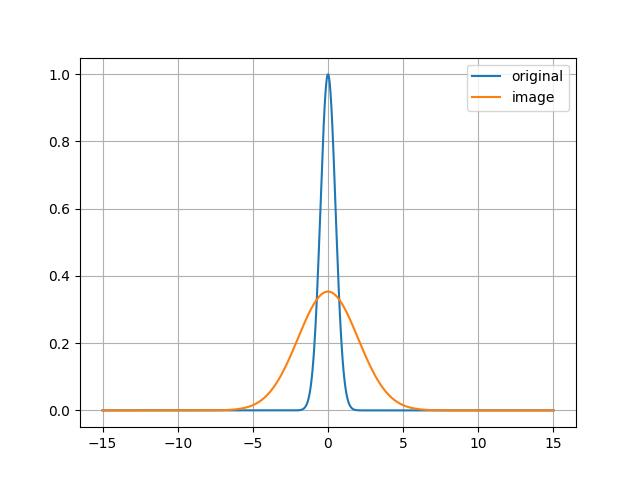
\includegraphics[width=\linewidth]{../image/gauss_function_1_2.jpg}
      \caption{$a=1$, $b=2$}
    \endminipage\hfill
    \minipage{0.32\textwidth}
      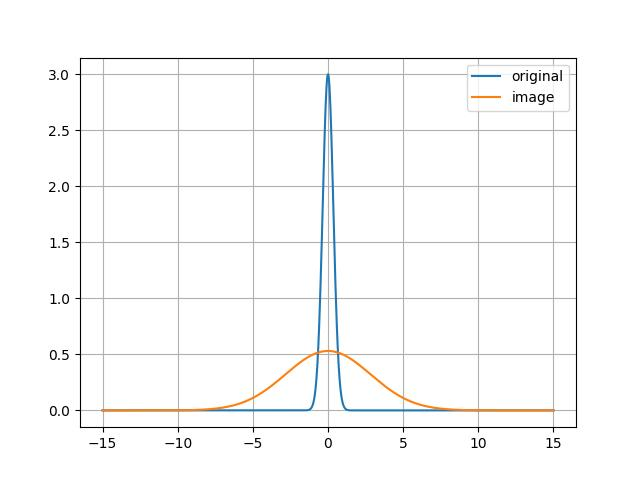
\includegraphics[width=\linewidth]{../image/gauss_function_3_4.jpg}
      \caption{$a = 3$, $b = 4$}
    \endminipage\hfill
    \minipage{0.32\textwidth}%
      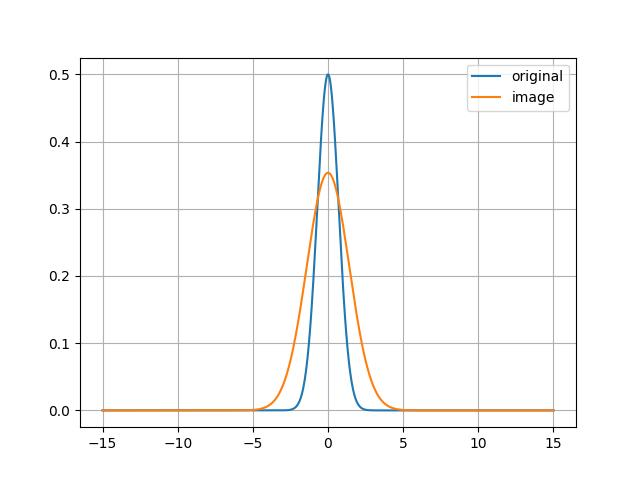
\includegraphics[width=\linewidth]{../image/gauss_function_0.5_1.jpg}
      \caption{$a = 0.5$, $b = 1$}
    \endminipage
    \end{figure}
    \newpage
  \subsection{Двустороннее затухание}
  \[
  f_5(t) = 
    a e^{-b|t|}
  \]
  \textbf{Образ Фурье:}  \\
  \begin{center}
    $c_5(\omega) = \frac{1}{\sqrt{2\pi}} \int\limits_{-\infty}^{+\infty}f(t)e^{-i\omega t}dt = 
  \frac{1}{\sqrt{2\pi}} a \int\limits_{-\infty}^{+\infty} e^{-b|t| - iwt}dt  
  $ 
  \end{center} 
  \begin{center}
  $c_5(\omega) = 
  \frac{a}{\sqrt{2\pi}} \int\limits_{-\infty}^{0}e^{t(b - i\omega)}dt + \frac{a}{\sqrt{2 \pi}} \int\limits_{0}^{+\infty} e^{-t(b + i \omega)}dt=
  \frac{a}{\sqrt{2 \pi}}(\frac{1}{b-i\omega} + \frac{1}{b+i\omega}) = \frac{a}{\sqrt[2]{2 \pi}}\frac{2b}{b^2 + \omega^2} = 
  \sqrt{\frac{2}{\pi}}\frac{ab}{b^2+\omega^2}
  $
  \end{center}
  \noindent \textbf{Равенство Парсеваля:}
  \begin{center}
    $\parallel f \parallel^2 = \int\limits_{-\infty}^{+\infty} f^2(t) dt= [a = 1, b = 3] = \frac{1}{3}  $
  \end{center}
  \begin{center}
    $\parallel c(\omega)\parallel^ 2 = \int\limits_{-\infty}^{\infty}c^2(\omega)d\omega = \frac{1}{3}$
  \end{center}
  \begin{figure}[!htb]
    \minipage{0.32\textwidth}
      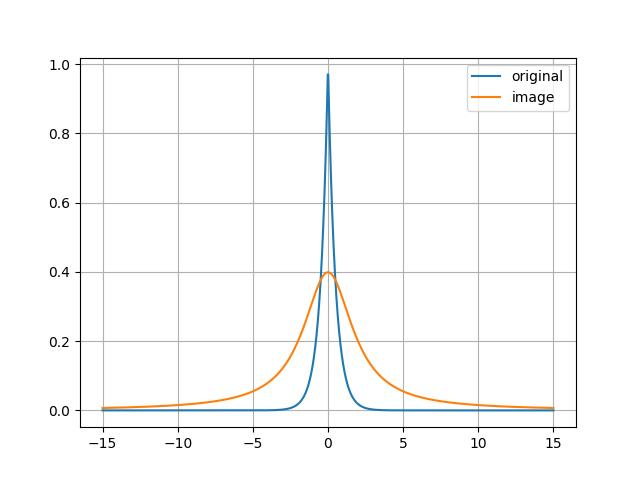
\includegraphics[width=\linewidth]{../image/two_way_attenuation_function_1_2.jpg}
      \caption{$a=1$, $b=2$}
    \endminipage\hfill
    \minipage{0.32\textwidth}
      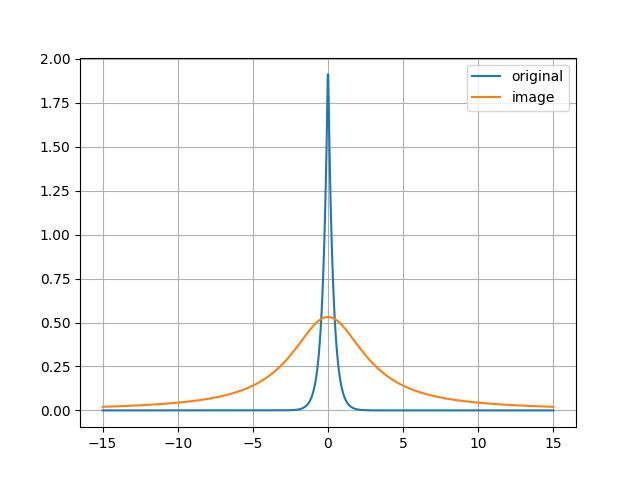
\includegraphics[width=\linewidth]{../image/two_way_attenuation_function_2_3.jpg}
      \caption{$a = 2$, $b = 3$}
    \endminipage\hfill
    \minipage{0.32\textwidth}%
      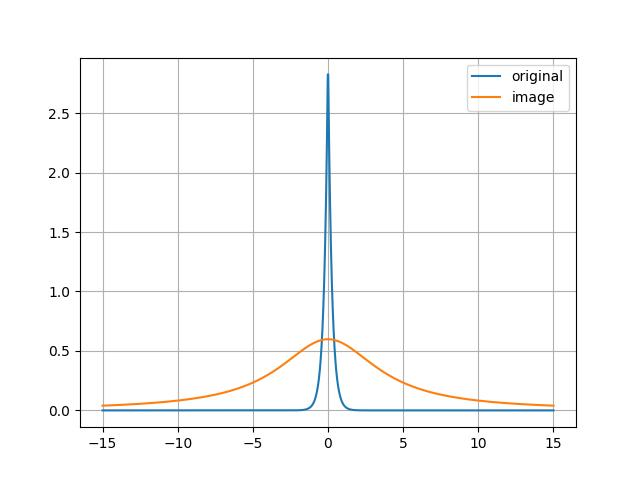
\includegraphics[width=\linewidth]{../image/two_way_attenuation_function_3_4.jpg}
      \caption{$a = 3$, $b = 4$}
    \endminipage
    \end{figure}
    \subsection{Общий вывод}
    \noindent По графикам видно, что $a$ отвечает за растяжение вдоль оси $Oy$, $b$ - вдоль оси $Ox$. В более менее классической формулировке принцип неопределенности удтверждает, что для неккоммутируемых величин(т.е коммутатор не равен нулю - операторы положения и импульса подходят, например - их коммутатор равен $i\frac{h}{2\pi}$) существует предел точности одновременного измерения. Иначе говоря, мы не можем знать положение и импульс частицы в один момент времени без погрешности. Чем точнее знаем импульс, тем хуже положение (и наоборот).
 Т.к частицу можно описывать волновыми характеристиками (принцип
 корпускулярно-волнового дуализма), то как я понимаю наш случай с функциями и их
 образами, графики функций - функция плотности распределения положения частицы.
 То есть чем больше площадь под синим (в моем случае) графике, тем больше точек,
 в которых частица может быть обнаружена с ненулевой вероятностью.
 Чем больше ж еплощадь под графиком фурье образа, тем больше погрешность измериений импульса частицы. И когда мы уменьшаем площадь под одним из графиков, то увеличивается площадь по вторым (и наоборот).
    \section{Комплексное}
  \subsection{Процесс}
  \noindent Возьмем функцию двустороннего затухания. Зафиксируем $a = 2$, $b = 4$
   \[
  f(t) = 2e^{-4|t|}
  \]
  \[
  g(t) = f(t + c) = 2e^{-4|t+c|}  
  \]
  \begin{center}
    $\hat{g}(t) = \frac{1}{\sqrt{2\pi}} \int\limits_{-\infty}^{+\infty}f(t+c)e^{-i\omega t}dt = [t+c = \mu]=
  \sqrt{\frac{2}{\pi}}\int\limits_{-\infty}^{+\infty}e^{-4|\mu|} e^{-iw(\mu-c)}d\mu 
 =
  e^{iwc} \sqrt{\frac{2}{\pi}}(\int\limits_{-\infty}^{-c} e^{(4 - iw)\mu}d\mu + \int\limits_{-c}^{\infty} e^{-(4 + iw)\mu}d\mu)
  =
  e^{iwc} \sqrt{\frac{2}{\pi}}(\frac{1}{4-iw}e^{-c(4-iw)} + \frac{1}{-(4+iw)}e^{c(4+iw)})
  $ 
  \end{center} 
  Также построим графики сдвинутой функции и её Фурье образа
  \newpage
  \begin{figure}[!htb]
    \centering
      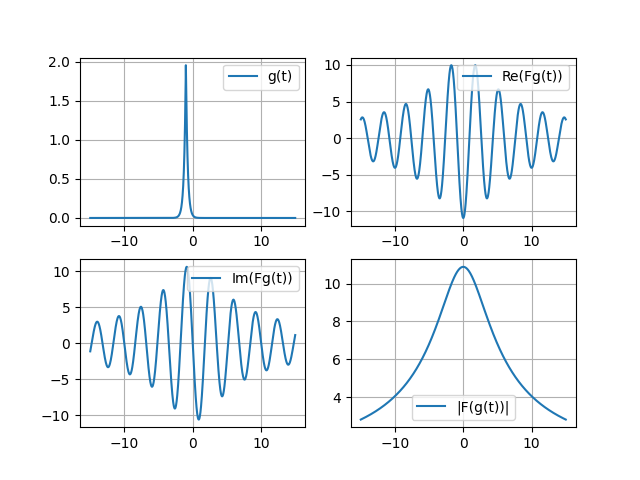
\includegraphics[scale=0.7]{../image/complex_case_img/com_1'.png}
      \caption{$c=1$}
  \end{figure}
  \begin{figure}
    \centering
      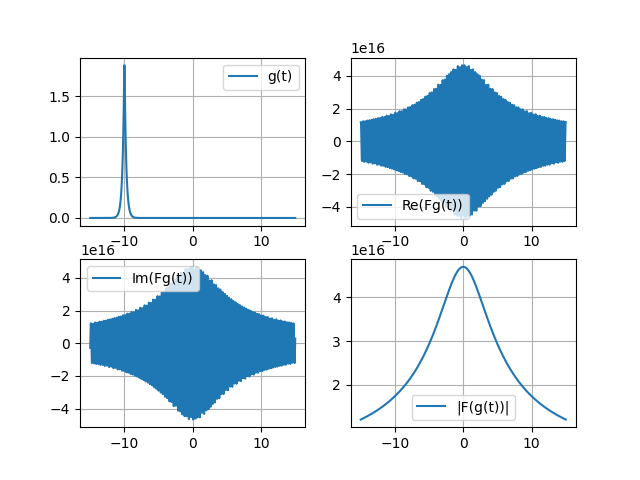
\includegraphics[scale=0.9]{../image/complex_case_img/com_10.png}
    \caption{$c=10$}
    \end{figure}
  \begin{figure}
    \centering
      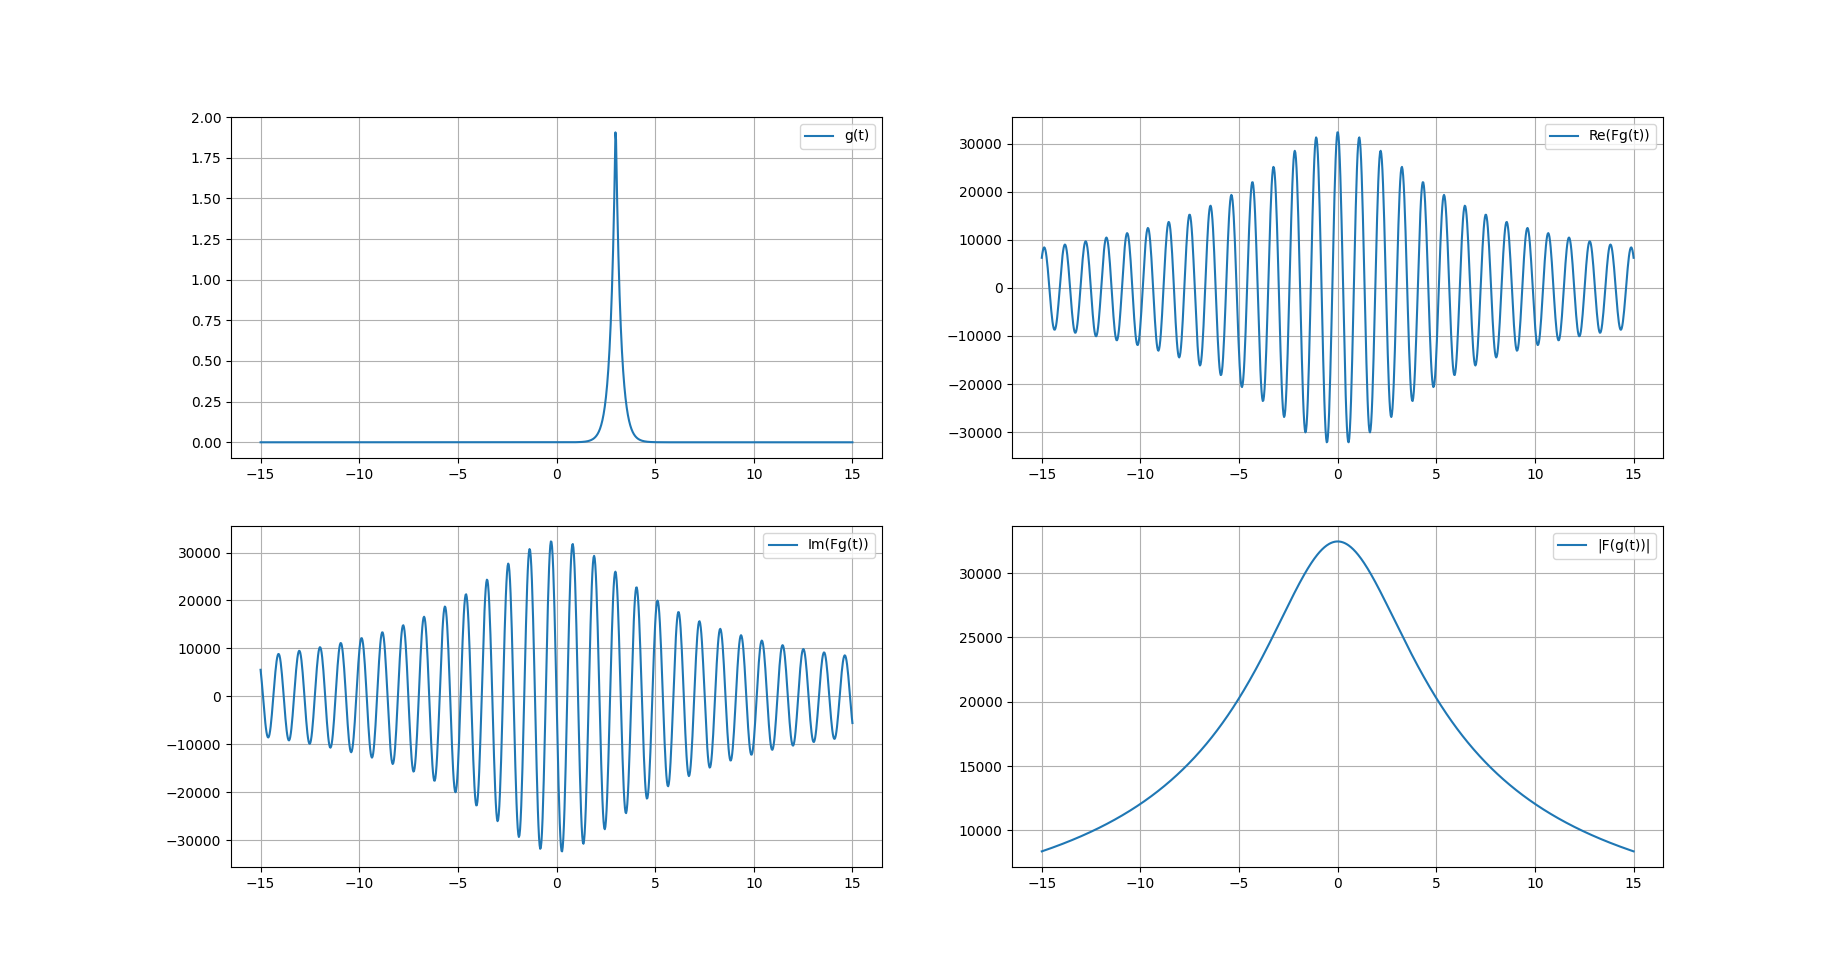
\includegraphics[scale=0.4]{../image/complex_case_img/com_-3.png}
      \caption{$c=-3$}
  \end{figure}
  \clearpage
\newpage
  \subsection{Вывод}
  \noindent Влияние параметра c на саму функцию достаточно предсказуемо - параметр отвечает за сдвиг функции, чем он больше - тем дальше, направление сдвига зависит от знака c. На фурье образ влияние более интересное - чем больше модуль параметра, тем чаще колеблется вещественная и мнима часть образа. Если же построить образ на комплексной плоскости, мы должны пронаблюдать большее количество вращений при увеличении модуля c.
  \section{Музыкальное}
  \noindent На этот раз откроем Matlab, напишем простую программу, которая выведет график, на котором по оси X будут отображаться частоты в герцах, а на оси Y - <<вовлеченность>> частоты в  аккорд. 
   \begin{lstlisting}
  [y,f] = audioread("n15.mp3"); y = y(:,1);
  dt = 1/f; 
  T = length(y) * dt;
  
  t = 0:dt:T;
  t = t.';

  dv = 1;
  v = 0 : dv : 1000;
  Y = zeros(1,length(v));
  for k = 1 : length(v)
      Y(k) = trapz(y.*exp(-1i*2*pi*v(k)*t));
  end

  plot(abs(Y));
  \end{lstlisting}
  \begin{figure}[!htb]
    \minipage{0.29\textwidth}
      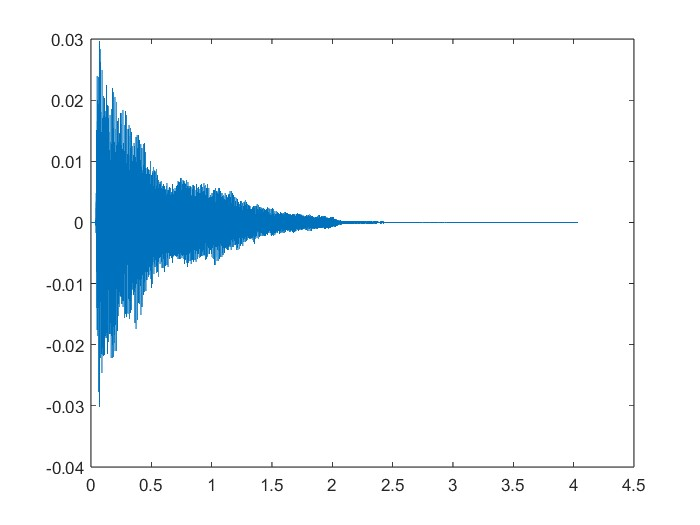
\includegraphics[width=\linewidth]{../image/music_case_imgs/soundwave.jpeg}
      \caption{Аккорд-15}
    \endminipage\hfill
    \minipage{0.7\textwidth}
      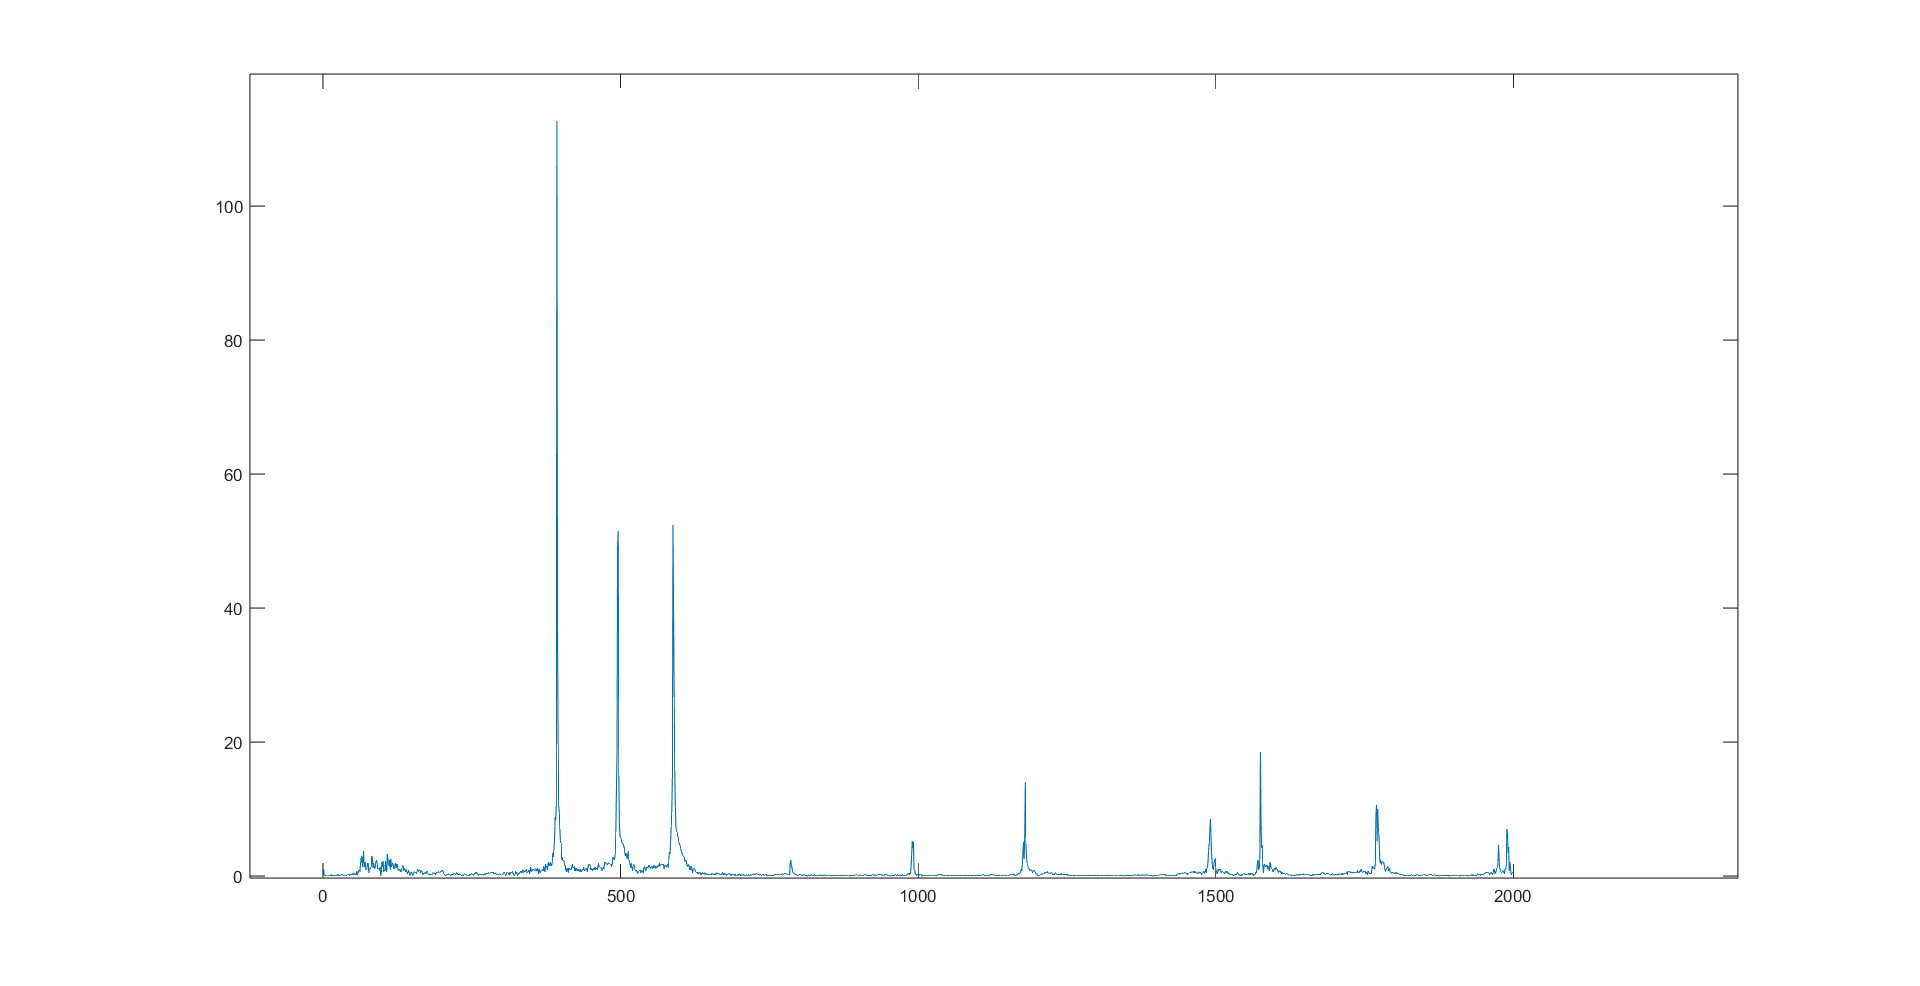
\includegraphics[width=\linewidth]{../image/music_case_imgs/hist_music.jpg}
      \caption{Распределение частот аккорда}
    \endminipage\hfill
    \end{figure}
  На графике имеем три пика на следующих частотах: 588, 495, 393. Значит аккорд №15 состоит из таких нот, как: Ре(2ая октава), Си(1ая октава), Соль(1ая октава).
  \end{document}
  